% Implementierung

\chapter{Implementierung}
\label{implementierung}

\section{Aufbau Struktur des Projektes}

Wie im Kapitel \ref{konzept} erläutert stellt mARt jeweils eine zwei- und dreidimensionale Darstellung der MRT-Daten zur Verfügung, zwischen denen gewechselt werden kann. Auf Grund der beschriebenen Hindernisse bezüglich der Leistungsfähigkeit der Hololens, wurde die Anwendung sowohl für die Hololens als auch als VR-Anwendung implementiert. Die AR-Anwendung bietet dabei nicht die volle Funktionalität und stellt die dreidimensionale Visualisierung nur beispielhaft dar. Die VR-Anwendung ermöglicht dagegen eine interaktive Echtzeit-Darstellung des Volumens. In beiden Fällen handelt es sich allerdings im Kern um die selbe Anwendung, d.h. die Software sollte für beide Gräte entwickelt werden. 
Sowohl für die Entwicklung von VR- als auch AR-Anwendungen werden im Allgemeinen GameEngines verwendet, da sie als Oberfläche diesen, um interaktive 3D-Anwendungen zu erzeugen, die in Echtzeit funktionieren. 
Zur Implementierung von mARt wurde \textit{Unity} von \cite{unity} verwendet. Die Engine gehört zu den meist genutzten auf dem Markt. Laut \cite{unityRelations} selbst, werden 60\% von AR/VR Inhalten mit Unity entwickelt. Weiterhin ermöglicht Unity die Entwicklung von Software für die meisten Plattformen. Unity bietet viele nützliche Funktionen zur Entwicklung von interaktiven Anwendungen und wird außerdem von einer großen  Gemeinschaft genutzt, sodass neben einer detaillierten Dokumentation auch über Foren und Webartikel hilfreiche Informationen zur Entwicklung zur Verfügung stehen.

Microsoft empfiehlt weiterhin Unity zur Entwicklung für Hololens-Software zu nutzen \cite{unityHololens} und bietet mit \textit{Mixed Reality Toolkit} (MRTK) \cite{holoToolkit} ein Framework, das Hololens Funktionen innerhalb von Unity zur Verfügung stellt.
Unity verwendet C\# als Skriptsprache, was vor allem den Einstieg in die Programmierung erleichtert. Die Engine selbst ist allerdings in C++ geschrieben, wodurch effiziente Berechnungen zur Laufzeit ermöglicht werden.
%Wieso?

mARt wurde in Unity entwickelt und sollte dann sowohl für die HoloLens und als VR-Anwendung gebaut werden. Die Anwendung konnte allerdings nicht für die HoloLens bereitgestellt werden. Diese Problematik wird in Abschnitt \ref{kombination} erläutert. Auf die Entwicklung für die unterschiedlichen Plattformen wird im Abschnitt \ref{plattformen} näher eingegangen.

Um die Unity Anwendung auf dem VR-System abzuspielen, wird die \textit{SteamVR}-Software von \citep{steam} in das Projekt integriert. Um die Anwendung starten zu können muss sie auf dem jeweiligen Rechner installiert sein.

\subsection{Unity Projekt}

Unity Projekte basieren auf 3D-Szenen. Innerhalb einer Szene können GameObjects platziert werden. Dabei kann es sich z.B. um 3D-Modelle handeln. Ein GameObject besitzt verschiedene Components, die dessen Eigenschaften und Verhalten bestimmen. Viele Funktionen und Eigenschaften werden von bereits in der Engine vorhandenen Components realisiert. Sogenannte Rigidbodys verleihen einem Objekt beispielsweise physikalische Eigenschaften, die von der Engine berechnet werden. Components können auch Skripte sein, die der Entwickler selbst verfasst hat. Über diese Skripte wird die Spiellogik und die Funktionalität der Anwendung definiert. 

Da mARt sich hauptsächlich in die beiden Szenarien einer zwei- und dreidimensionalen Darstellung unterteilen lässt existiert für jedes Szenario eine Szene.
Viele der Funktionen sind allerdings ähnlich oder gleich, weshalb manche Skripte in beiden Szenen verwendet werden. 


\section{Implementierung verschiedener Technologien/Plattformen}
\label{plattformen}

\subsection{HoloLens Prototyp}
Im Rahmen der Arbeit wurde neben der endgültigen Anwendung zuerst auch eine prototypische Demo-Anwendung entwickelt, die die Hololens eigenen Gesten genutzt hat. Die Anwendung hat eine zweidimensionale Darstellung der MRT-Bilder als Hologramm in den Raum projiziert, welches der Nutzer durch Hololens eigene Gesten manipulieren konnte. Dabei wurden alle vorhandenen Manipulierungsformen eines Hologramms abgedeckt, sowie das Scrollen durch die Bildschichten. Um die Hololens Gesten zu Nutzen wurde das HoloToolkit verwendet. 
Anhand dieser Demo sollte geprüft werden, ob die Interaktionsmöglichkeiten, die die Hololens bietet ausreichend sind, um einem Neurologen die effektive Untersuchung von MRT-Bildern zu ermöglichen.
Weiterhin konnten durch das Testen einer realen Anwendung die Erwartungen und Anforderungen eines Arztes an mARt noch weiter spezifiziert werden.  

Wie im Kapitel \ref{konzept}erläutert, haben sich die Gesten der Hololens zwar als ausreichend erwiesen, machten aber die Verwendung von weiteren Bedienelementen notwendig, z.B. zum Wechseln der Manipulationsart. Aus den beschriebenen Gründen wurde für die endgültige Implementierung der Anwendung die Motion Leap in das System integriert.
% Genauer auf Implementierung eingehen

\todo{Bild von Demo}

\subsection{HoloToolkit}

HoloToolkit, Input, Camera etc
\section{Implementierung der Nutzereingabe}
Steam VR, normale scene

\subsection{Leap Motion}

Damit die Motion Leap Kamera in einer Anwendung verwendet werden kann, muss das von \cite{orion} zur Verfügung gestellte SDK \textit{Orion} eingebunden werden. Das \textit{Core SDK} ist dabei zur Erkennung und Verwendung des Gerätes notwendig, während ein erweiterndes Paket für Interaktionen die Funktionen und Beispiele bietet, wie verschiedene Bedienelemente in eine Anwendung integriert werden können, die auf die Controller, also die Hände des Nutzers reagieren.
Meistens funktioniert dies indem einzelne Skripte, die das gewünschte Verhalten implementieren als Components an GameObjects angehangen werden. Die Skripte lösen dann bestimmte Events oder Methoden aus, die mit den Funktionalitäten der Anwendung verknüpft werden. 

\subsection{Kombination von Leap Motion mit Vive/Hololens}
\label{kombination}

Sowohl Vive als auch HoloLens sollen in Verbindung mit der Leap Motion funktionieren. Dazu muss zum Einen die Leap Motion Kamera in beide Systeme integriert werden und zum Anderen die Funktionalität in die Unity jeweiligen Szenen eingebaut werden. 

Das Einbinden der Leap Motion in eine VR Anwendung, sowie die Kombination mit dem HTC Vive Headset sind unproblematisch. Das Orion SDK der Leap Motion unterstützt den Einsatz in VR-Szenen. Sofern SteamVR installiert und eine VR-Brille angeschlossen ist, ist kein größerer Aufwand nötig, um die Hände des Nutzers in VR anzuzeigen. 
Die Integration in das VR-System ist vergleichbar einfach. Die Leap Motion Kamera wird vorne auf dem HMD über der eingebauten Kamera befestigt und ihre Kabel zusammen mit den anderen der Brille über den Kopf des Nutzers geführt. 

Dagegen bringt die Verbindung von Motion Leap und Hololens einige Herausforderungen mit sich. Zunächst ist in einer Hololens-Szene nur eine Kamera, die des HMDs, vorgesehen. Das Vorhandensein einer zweiten Kamera, wie die der Leap Motion würde beim Erstellungsprozess zu Fehlern führen,sodass das Bereitstellen des Programmes für die Hololens nicht möglich ist.
Die Leap Motion wird über ihr Kabel mit Strom versorgt. Sie kann also im Gegensatz zu der Hololens nicht kabellos funktionieren. 
Über das Kabel werden außerdem die von der Leap Motion Kamera erfassten Daten weitergeleitet, die dann verarbeitet werden. Die dafür notwendige Software ist nicht für die Hololens verfügbar und es ist fragwürdig, ob sie die dafür notwendige Rechenleistung besitzt. 

Aus diesen Gründen muss die Leap Motion während des Betriebs per Kabel mit einem Rechner verbunden sein. Um das Gerät trotzdem in Verbindung mit der Hololens nutzen zu können, müssen entweder die Sensordaten der Leap Motion an die Anwendung in der Hololens übertragen werden oder die gesamte Anwendung läuft auf dem Rechner und wird zur Wiedergabe an die Hololens übermittelt. Beides geschieht über Wlan.

Die Übertragung der Sensordaten ist dabei um einiges aufwändiger und erfordert die Integration weiterer Tools. Es existieren einige Lösungsansätze für dieses Problem, beispielsweise von \cite{hololensGithub}. Auf Grund des beschränkten Zeitraums dieser Arbeit wurde dieser Ansatz allerdings nicht implementiert.
Stattdessen wird die Anwendung lediglich auf der HoloLens wiedergegeben. Dazu wird die Hololens-App \textit{Holographic Remoting Player} von \cite{remoteApp} genutzt. Die Anwendung wird dabei direkt aus dem Unity-Editor übertragen.
Die Wiedergabequalität der Anwendung ist dabei abhängig von der Stabilität der Wlan-Verbindung.

Auch das Anbringen der Leap Motion an das HMD ist bei der HoloLens umständlicher als bei der HTC Vive. 
Da es die Vive einen undurchsichtigen Bildschirm besitzt, kann die Leap Motion Kamera einfach vorne auf der Brille befestigt werden. Die Form des Gerätes bietet dazu ausreichend Fläche.
Bei der HoloLens sollte der Bildschirm, durch den der Nutzer sieht nicht verdeckt werden. Eine Installation  im oberen Teil der Frontseite ist ebenfalls nicht umsetzbar, da dieser von den HoloLens-Kameras eingenommen wird, die die Umgebung und Nutzergesten verfolgen.
Somit ist die einzige sinnvolle Möglichkeit, die Leap Motion auf der HoloLens zu platzieren. Hierbei muss sie außerdem nach vorne geneigt werden, um die Hände des Nutzers in der Anwendung möglichst genau an den realen Händen auszurichten. 
Um die Anwendung auf der HoloLens bedienen zu können, wurde eine eigene Haltungsvorrichtung gebaut.

\todo{Foto von Halterung?}


\section{Shader in Unity}

Wie in Kapitel \ref{konzept} beschrieben, wird das Volume Rendering der MRT-Daten in einem Shaders umgesetzt. An dieser Stelle soll ein Überblick über die Funktionsweise und den Aufbau von Unity-Shadern gegeben werden. 

Wie ein Objekt in einer Szene gerendert wird hängt in Unity davon ab, welches Material diesem zugewiesen ist. Das Material fungiert dabei als eine Art Behälter für sämtliche Parameter, die das Aussehen des Objektes beeinflussen, wie z.B. die Textur oder Farbe. Welche Parameter das Material besitzt und wie diese miteinander verrechnet werden bestimmt der Shader des Materials. Innerhalb des Shaders wird in Abhängigkeit zu den diesem übergebenen Werten die Farbe für jeden Pixel errechnet. 
% https://docs.unity3d.com/Manual/Shaders.html

Shader in Unity sind in der Unity eigenen Shader-Sprache \textit{Shader Lab} geschrieben. Im Shader ist definiert, welche Eigenschaften dieser besitzt und welche Sub- und Fallback-Shader er verwendet.
Die Eigenschaften sind die eben genannten Parameter, dessen Werte dann über das Material gesetzt werden. Hier werden deren Namen, Typen, ihr Wertebereich, sowie ihre Standardwerte definiert. 

Schließlich werden im Shader auch sogenannte Subshader definiert, die den eigentlichen Shader-Code enthalten.
Ein Shader kann mehrere Subshader enthalten für den Fall, dass einer der Shader von einem Gerät nicht unterstützt wird. Wird keiner unterstützt wird der Fallback-Shader verwendet. 
Neben dem Shader-Code besitzt ein Subshader Tags, die bestimmen, wann und wie ein Shader von der Rendering Engine gerendert werden soll. Dies kann sich beispielsweise auf die Reihenfolge beziehen, in der Objekte gerendert werden oder ob ein Objekt Schatten werfen soll. 
Nach den Tags folgt die Definition eines \textit{Pass}. Als Render Pass wird der gesamte Prozess bezeichnet, der durchlaufen wird, um einen Pixel zu rendern. Angefangen bei der Berechnung einzelner Vertices eines Meshes über den Vertex-Shader bis zum Fragment-Shader. D.h. im Pass werden in verschiedenen Methoden die tatsächlichen Berechnungen beschrieben, die zum Aussehen jedes Pixels führen. 
Auch ein Pass kann zunächst wieder Tags enthalten, die bestimmen wann oder wie oft ein Pass durchlaufen werden soll. 
% Render setup ????
Dann folgt der Code Abschnitt, der den Shader-Code enthält. Dieser ist in Cg (C for Graphics)
\todo{REFERENZ} geschrieben, einer Shading-Sprache, die syntaktisch stark HLSL (High-Level Shading Language) ähnelt. 
Abhängig davon, um welche Art von Shader es sich handelt werden hier die notwendigen Funktionen implementiert. Unity besitzt sogenannte Surface-Shader, ein vereinfachter Shader, für den kein Beleuchtungsmodell implementiert werden muss. Andererseits können auch Vertex-Fragment-Shader implementiert werden, die auch Unlit-Shader heißen. 

Das Volume Rendering der MRT-Daten erfolgt durch einen Vertex-Fragment-Shader auf die genaue Implementierung wird im Folgenden eingegangen. 

% https://docs.unity3d.com/Manual/SL-Shader.html
\todo{
-Was is cg hlsl?
- Was sind compute, surface, unlit shader?
- Graphic pipeline?
REFERNZEN
}
\section{Grundlage}

Die in Kapitel \ref{anforderung} beschriebenen Anforderungen stellen den Umfang der zu implementierenden Anwendung dar. 
Neben der Umsetzung der Anwendungslogik stellt vor allem die Implementierung der 3D-Darstellung durch Ray-Casting einen hohen Aufwand dar. Um diesen in einem realisierbaren Rahmen zu halten, wurde ein bereits existierendes Programm als Basis für die zuletzt genannte Funktionalität verwendet.
Wie in Kapitel \ref{grundlagen} beschrieben wurde, gibt es bereits viele Implementierungen von Volume Ray-Casting zur Visualisierung von medizinischem Bildmaterial. 
Die dort genannten Unity-spezifischen Lösungen sind allerdings kostenpflichtig und/oder ihre Codebasis ist nicht einsehbar. Es wäre allerdings von Vorteil die Kontrolle über die Implementierung der 3D-Darstellung zu haben, um so die Möglichkeit zu haben, sie den Anforderungen entsprechend anpassen zu können.
Aus diesem Grund wurde die Open-Source-Implementierung von \cite{volumeRenderingGit} als Grundlage für die 3D-Darstellung verwendet. 
Diese wurde erweitert, um die Anforderungen an mARt zu erfüllen. 
Im Rahmen der Arbeit wurden folgende Bestandteile implementiert:

\begin{itemize}
\item Erweiterung des Shaders (Maske, Beleuchtung)
\item Umwandlung von Bilddaten in 3D-Texturen und der Berechnung ihrer Gradienten
\item Anpassung der Bedienelemente an 3D-Szene
\item Anwendungslogik
\end{itemize}
Der verwendete Code ist im Projekt markiert.
\section{Volume Rendering}

Wie in Kapitel \ref{konzept} beschrieben, wurde der 3D-Darstellung des Gehirns mit Hilfe von Volume Ray-Casting umgesetzt. 

Im Kapitel \ref{grundlagen} wurde der theoretische Vorgang dieser Technik beschrieben. Dieser Abschnitt fokussiert sich auf die Implementierung der einzelnen Schritte.

Die volumetrische Darstellung des Gehirns wird im Grunde genommen mit nur 3 Skripten erzeugt. Zuerst wird in VolumeRendering.cs das Mesh des Würfeln generiert. Hier werden auch die Parameter aktualisiert, die für das Rendering relevant sind, wie z.B. die 3D-Textur oder Farbe, sowie die Parameter, die durch die Nutzerschnittstelle manipuliert werden können. 
Die Parameter werden an den Shader übergeben, in dem das Rendering definiert ist. Der Cg-Code, der den Vertex- und Fragmentshader implementiert ist dabei in ein eigenes Script ausgelagert.
\todo{Warum?}

\subsection{Ray Casting}

Im Fragment Shader des \textit{Volume\_DiffuseWITHMask.sh} 
\todo{umbenennen} wird zunächst ein Strahl definiert, der von dem aktuell betrachteten Vertex aus von der Kameraposition in die Welt "geschossen" wird. In einem selbst definierten struct werden die maximalen und minimalen Werte definiert, aus denen sich die Eckpunkte des dargestellten Würfeln zusammensetzten. Anschließend wird geprüft, ob der Strahl den Würfel schneidet. 

%-----------Intersect-----------
%Dies geschieht indem zuerst die Inverse der Strahlrichtung ermittelt wird. Die Inverse eines Vektors $v$ ist $v^-1$ und da $v^-x=\frac1}{v^x}$, ergibt sich die Inverse des Richtungsvektors des Strahls indem $1$ durch die dividiert wird.
% AABB, axis aligend etc? intersection formula REFERENZ
Um die Schnittpunkte des Strahls zu ermitteln nimmt man an, dass die sechs Seiten des Würfels auf jeweils sechs Ebenen liegen, wobei davon zwei immer parallel sind. Zuerst werden jetzt alle Schnittpunkte des Strahls mit diesen Ebenen berechnet und dann geprüft, ob die Schnittpunkte innerhalb des Würfels liegen.
Der Würfel wird durch zwei Eckpunkte beschrieben. Da der Würfel Koordinaten von -0,5 bis 0,5 hat können wir hierfür die jeweils kleinsten und größten Koordinaten nutzen. 
Die Schnittpunkte des Strahls, mit den x-, y- und z-Ebenen ergeben sich durch das Umstellen der Formel, die einen Strahl beschreibt:

\begin{align}
p=r_{Ursprung}+t*r_{Richtung}
\end{align}

$r_{Ursprung}$ ist dabei der Ursprung des Strahls und $r_{Richtung}$ seine Richtung. $p$ ist ein Punkt auf dem Strahl und $t$ ein Parameter, der bestimmt wie weit der Punkt vom Ursprung entfernt ist.

Um die Schnittpunkte mit den Ebenen zu erhalten wird die Formel nach $t$ umgestellt:

\begin{align}
t=(p-r_{Ursprung})/r_{Richtung}
\end{align}

Für $p$ werden jeweils die beiden Eckpunkte des Würfels, die jeweils auf drei der Würfelebenen liegen, eingesetzt.
Dadurch sind insgesamt sechs $t$s und damit sechs Schnittpunkte mit den Ebenen bekannt. Zwei auf jeder Ebene. Die Entfernungen werden in den zwei dreidimensionalen Vektoren $t_{unten}$ und $t_{oben}$ gespeichert. Durch den Vergleich der t-Vektoren wird festgelegt, welcher Eckpunkt und damit welche zweier paralleler Ebenen weiter vorne liegt. 
% Was wenn Strahl parallel zur Ebene ist??
Jetzt muss bestimmt werden, ob diese Schnittpunkte sich innerhalb des Würfels befinden.
Dazu werden jeweils die x-, y- und z-Werte der t-Vektoren untereinander verglichen. Für das $t$ der näher gelegenen Ebene wird der maximale, für den weiter entfernten der minimale Wert bestimmt. Ist der Wert des näheren $t$s größer als der des entfernten, schneidet der Strahl den Würfel nicht. Andersherum tut er es.
Das Verhältnis der Schnittpunkte zueinander und wie dieses durch den Verlauf des Strahls bestimmt wird ist in Abbildung \ref{img:rayBoxHit} dargestellt.

\begin{figure}[!htb]
	\centering
	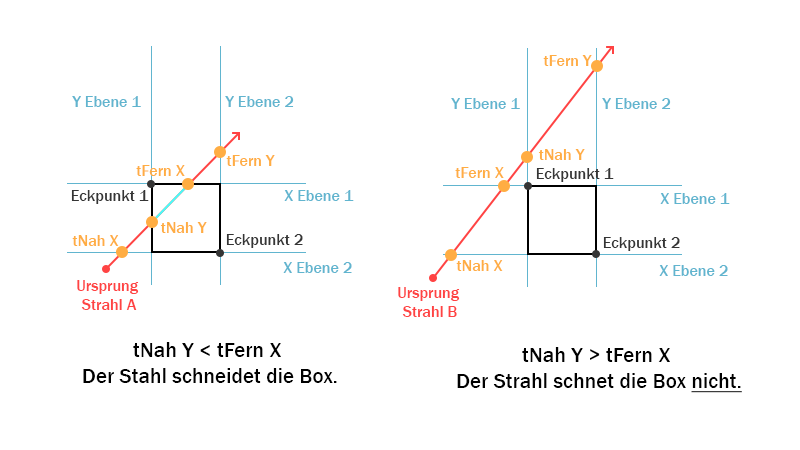
\includegraphics[width=0.9\linewidth]{images/rayBox.png}
	\caption{Zweidimensionale Darstellung, wie ein Strahl durch eine Box (links) und daran vorbei (rechts) verläuft. Die Schnittpunkte des Strahls (gelb) mit den Würfelebenen (blau) sind eingezeichnet. Der Vergleich derer Abstände zum Ursprung des Strahls (rot) zeigt, ob der Strahl die Box schneidet oder nicht.}
	\label{img:rayBoxHit}
	\source{Eigene Darstellung}
\end{figure}
\FloatBarrier

%----------------------------------------
Die beiden t-Werte werden als $t_{nah}$ und $t_{fern}$ gespeichert.
Mit dem Ursprung des Strahls und $t_{fern}$ werden Anfang, Ende und die Länge des Strahls berechnet. Mit Hilfe der Länge kann ermittelt werden um wie weit pro Iteration am Strahl entlang gegangen werden soll. Dadurch wird der Strahl nur bis zu seinem Austritt aus dem Würfel abgetastet. 

In einer for-Schleife wird jeder Strahl nun abgetastet. In jeder Iteration wird jeweils ein Punkt betrachtet. Der Punkt verschiebt sich entlang des Strahls um die zuvor berechnete Distanz.
Für jeden Punkt werden zuerst die uv-Koordinaten berechnet.

Für die Koordinaten werden dann die jeweiliges Isowerte aus der 3D-Textur gelesen, die zuvor mit den MRT-Bildern befüllt wurde.

%---------------SAMPLE VOLUME-------------
Hierbei werden lediglich die uv-Koordinaten als Indices für die Textur verwendet. 
Der Isowert ist dabei im Alphakanal der Textur gespeichert. Da es sich nicht um eine Farbe sondern nur einen Grauwert handelt, können die anderen Farbkanäle der Textur mit dem Gradienten des jeweiligen Pixels befüllt werden. Darauf wird im Abschnitt \ref{gradienten} genauer eingegangen.

Der Isowert wird außerdem noch mit der Intensität multipliziert, die der Nutzer beeinflussen kann.
\todo{Mit ergebnis abgleichen}
An dieser Stelle wird aber auch geprüft, ob der betreffende Punkt überhaupt zu sehen ist, oder aufgrund der verschiebbaren Schichten nicht sichtbar sein sollte. 
Dazu wird zuerst der aktuell betrachtete Punkt mit der Rotationsmatrix des Modells multipliziert.
\todo{ UBERPRÜFEN Warum?}
Der Punkt wird dann mit den minimalen und maximalen x-, y-, und z-Werten der verschiebbaren Schicht verglichen. Das Ergebnis des Vergleichs wird dabei in einer Variable gespeichert. Ist der Punkt kleiner als das Minimum oder größer als das Maximum wird 0 gespeichert, ansonsten 1. 
Die beiden Werte werden anschließend mit dem Isowert multipliziert.Ist einer der Werte null, ist auch der ermittelte Isowert null, was im Alphakanal totale Transparenz bedeutet. 
Das Ergebnis dieser Berechnung wird zunächst für jedem Farbkanal zugewiesen.
%-----------------------------------------

An dieser Stelle wird über die Transferfunktion der entsprechende Farbwert aus der zugehörigen Textur gelesen. Dazu wird der Isowert als Index verwendet. Die Funktionsweise und Implementierung der Transferfunktion wird in der Sektion \ref{transfer} beschrieben.
% Bezug Transferfunktion!
Die Transferfunktion wird nur abgerufen, wenn der Isowert nicht 0 ist, da sonst die Transparenz überschrieben würde.
% Tranferfunktion bei index 0 auf 0000 setzen??
Ist die Farbe bekannt, wir der betrachtete Voxel illuminiert. Dies ist in der Sektion \ref{ilumination} beschrieben. 

Der Alphawert der so erhaltenen Farbe wird noch einmal halbiert, um die Darstellung semi-transparent erscheinen zu lassen.
% WARUM

Schließlich wird der erhaltene Farbwert mit den vorhergehenden verrechnet. Die Komposition erfolgt dabei von vorne nach hinten, da der Strahl in dieser Richtung abgetastet wird, wie folgt:
% Referenz GPU Gems

\begin{align}
\hat{C}_{i}=(1-\hat{A}_{i-1})C_{i}+\hat{C}_{i-1}
\end{align}
\begin{align}
\hat{A}_{i}=(1-\hat{A}_{i-1})A_{i}+\hat{A}_{i-1}
\end{align}

Wobei $\hat{C}_{i}$ die Farbe und $\hat{A}_{i}$ die Transparenz der Farbe des vordersten Voxels ist.
Wenn diese Farbe einen vorher definierten Schwellenwert überschreitet wird die Schleife abgebrochen. Der Schwellenwert kann vom Nutzer manipuliert werden und bestimmt die ?Helligkeit? der Darstellung.

Die Farbe wird schlussendlich noch auf einen Wert zwischen 0 und 1 festgesetzt und mit der Farbe der Maske verrechnet, die auf dem selben Weg bestimmt wurde.

\subsection{Transferfunktion}
\label{transfer}

\todo{mit ergebnis abgleichen}

Um eine Transfertextur zu erzeugen, werden zunächst zwei Key-Value-Listen definiert, in denen bestimmte Isowerte einem Farb- oder Opazitätwert zugewiesen werden. In einem vom Rest der Anwendung unabhängigen Skript wird aus diesen einzelnen Punkten eine Textur erzeugt, indem zwischen den festgelegten Werten eine Interpolation stattfindet.
\todo{welche interpolation?}
Die Textur wird dann als 2D-Textur abgespeichert. Da allein die Isowerte als Index für die Zuordnung wurden, handelt es sich eigentlich um eine eindimensionale Transferfunktion. 
Allerdings werden von Unity keine 1D-Texturen als Shader Eigenschaften unterstützt. Da die Verwendung einer 2D-Textur aber keine Nachteile aufweist, wird stattdessen eine 2D-Textur verwendet, die eine einzige Y-Koordinate besitzt. 
Die Textur wird dann über das Material an den Shader übergeben. Wie im Abschnitt \ref{transfer} beschrieben, wird die Textur dann mit Hilfe eines Index' ausgelesen.

\subsection{Illumination}
\label{illumination}

Das Volumen wird mit mit dem Phong Beleuchtungsmodell illuminiert, wodurch es mehr Plastizität erhält. Das Modell wurde bereits in Kapitel \ref{grundlagen} detailliert beschrieben. Deshalb wird an dieser Stelle nur auch die Umsetzung im Shader eingegangen.
% Referenz? warum nicht blinn?
Wie beschrieben setzt sich das Modell aus drei Komponenten zusammen: Der ambienten und der diffusen Beleuchtung, sowie der spiegelnden Reflexion. Die Komponenten werden zusammen addiert, was in die endgültige Farbe resultiert. 
Die Koeffizienten werden im Shader durch Farben repräsentiert. Der diffuse Koeffizient ist dabei der vorher aus der Transferfunktion gelesene Farbwert. Um diesen nicht durch die ambiente Beleuchtung zu verfälschen, wird er mit einem konstanten Faktor multipliziert, um eine abgedunkelte Farbe zu erhalten, die als ambienter Wert verwendet wird. Die Reflextion wird weiß dargestellt.
%Als Reflexionsexponent hat sich der Wert ?10? als am besten erwiesen.

Um die Reflexion berechnen zu können müssen außerdem der Lichtvektor und die Normale bekannt sein.
Wie bereits erläutert, wird der Gradient eines Voxels als Normale verwendet. 
Der Vektor zum Licht wird aus der in Unity eingebauten Shader-Variable \textit{\_WorldSpaceLightPos0} ausgelesen.
Unterscheidung direktionales und Punktlicht?

\subsection{Gradientenberechnung}
\label{gradienten}


Die Gradienten werden vor dem Start der Anwendung berechnet und zusammen mit den Isowerten in eine 3D-Textur geschrieben. Der Gradientenvektor wird dabei in den RGB-Kanälen gespeichert und der Isowert im Alpha-Kanal, da es sich nur um einen einzelnen Wert handelt. 

Die Berechnung der Gradienten erfolgt im selben Schritt, wie das Übertragen der Skalarwerte aus den Bilddaten in eine 3D-Textur.
Dafür werden alle Bilddateien in einem Dateiverzeichnis auf das ein vorher definierter Pfad zeigt ausgelesen und in ein Array übertragen, das der Größe der Bilder entspricht. Die dritte Dimension des Arrays wird durch die Anzahl der Bilder bestimmt. 

Entsprechend der in Kapitel \ref{grundlagen} beschriebenen Finite-Differenzen-Methode, werden durch eine Convolution die Gradienten für jeden Farbwert berechnet und ebenfalls in ein Array gespeichert.
Das Gradientenarray wird anschließend mit Hilfe eines Gauß-Filters geglättet, bevor die Werte in eine 3D-Textur gespeichert werden. 

Diese wird im Assets-Verzeichnis des Projektes abgelegt. Sie werden in der Szene referenziert, um bei Bedarf an einen Shader übergeben zu werden, der den entsprechenden Datensatz darstellt. 